\section{Introduction}

Simulation-driven assessments and developments are a key method in various fields in industry and academia such as energy systems, production industry or social sciences. Due to the increasing complexity of systems, market competition, and specialization, it is harder to study the behavior of these systems. 
In order to keep reaping the benefits of simulation, new techniques to efficiently simulate the interactions between subsystems often built by  experts in different disciplines are required. There are two possibilities: (i) the entire system is modelled and simulated in a single tool which is referred to as monolithic simulation; or (ii) established tools for the respective subsystems are coupled in a so-called co-simulation. 

As our knowledge of each subsystem matures, modelling and simulation tools become more specialized, accumulating years of research and practical experience in their respective domains. 
As such, leveraging existing simulation tools, and coupling them in dynamic simulations---co-simulation---, provides a quick and accurate way to realize a holistic simulation by depicting interactions between subsystems while using the most appropriate simulators for each subsystem \cite{VanderAuweraer2013}. 
To assess developments and the importance of co-simulation in the scientific community in recent decades, a keyword analysis was conducted. 
The analysis was performed on \url{www.scopus.com} with the keyword ``co-simulation''. 
\Cref{fig:Publication} shows an almost linear growth of citations from $2000$ to $2017$. As it can be seen in Figure \ref{fig:Subject}, most of the publications are in the field of Engineering (40 \%) followed by Computer Science (25 \%) and Mathematics (11 \%).
Table \ref{tab:projects} gives an overview of research activities in the field of co-simulation in recent years.
%\claudio{I think we should move this paragraph to the previous section, as it motivates the other survey work also done. The current section aims at motivating our work by showing that it complements the existing survey work. Btw it should be clear what each section does and how they fit together.}

\begin{figure}[h!]
\centering
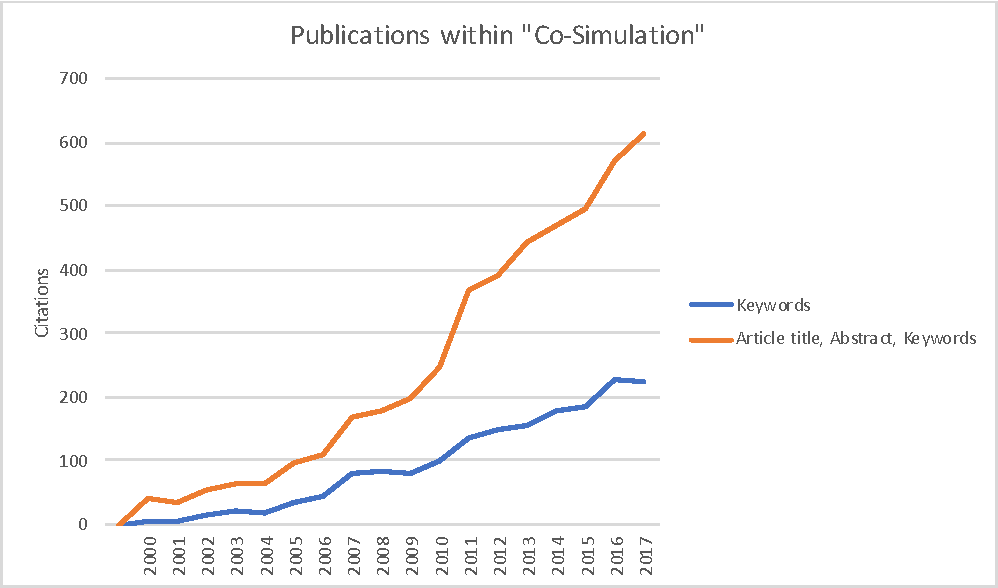
\includegraphics[width=1\textwidth]{Figures/Publications.pdf}
\caption{Publications with the keyword "co-simulation"}
\label{fig:Publication}
\end{figure}

\begin{figure}[h!]
\centering
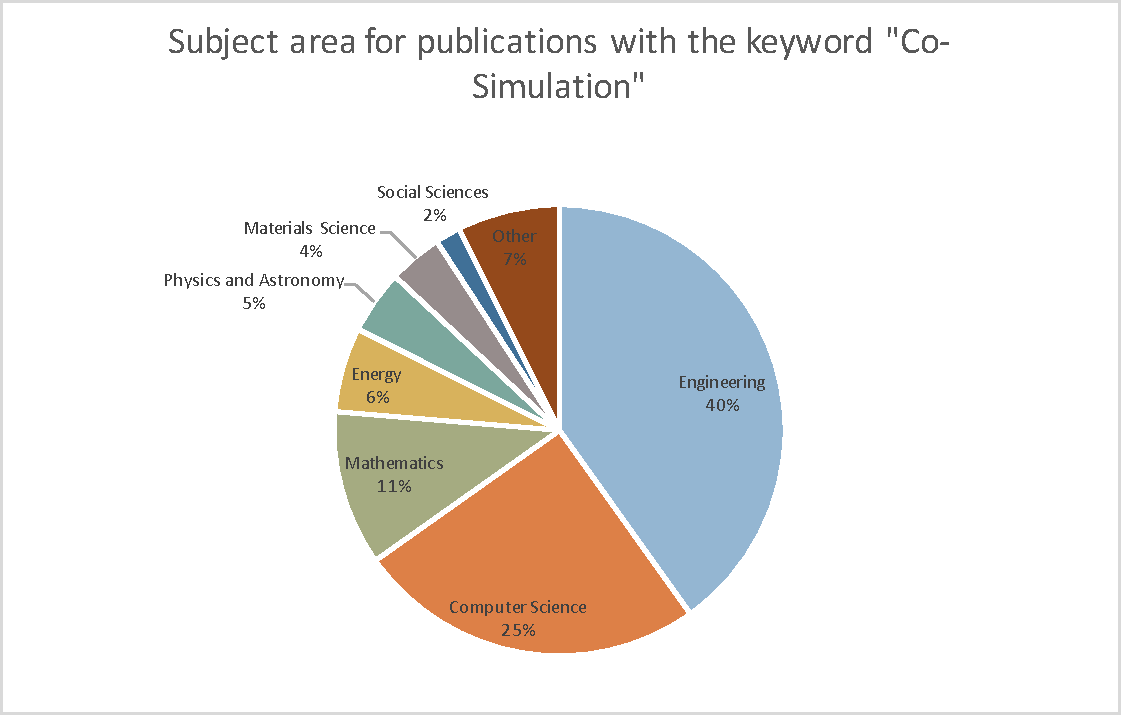
\includegraphics[width=1\textwidth]{Figures/Subject.pdf}
\caption{Subject area for publications with the keyword "co-simulation"}
\label{fig:Subject}
\end{figure}


% Please add the following required packages to your document preamble:
% \usepackage{graphicx}
\begin{table}[]
\caption{Research activities in the field of co-simulation in recent years}
\label{tab:projects}
\resizebox{\textwidth}{!}{%
\begin{tabular}{lll}
\textbf{Project name} & \textbf{Duration} & \textbf{Goals that relate to co-simulation} \\ \hline
COSIBA \cite{cosibas} & 2000 - 2002 & \begin{tabular}[c]{@{}l@{}}The aim was to formulate a co-simulation backplane for coupling electronic design automation tools, \\ that supports co-design using variousspecication formalisms at dierent abstraction levels.\end{tabular} \\
ODETTE \cite{odette} & 2000 - 20003 & \begin{tabular}[c]{@{}l@{}}The aim was to develop and market a complete co-design solution including hardware/software \\ co-simulation and synthesis tools.\end{tabular} \\
MODELISAR \cite{modelisar} & 2008 - 2011 & \begin{tabular}[c]{@{}l@{}}The aim was to improve the design of systems and of embedded software in vehicles. \\ One of the main results was the FMI standard.\end{tabular} \\
DESTECS \cite{destecs} & 2010 - 2012 & \begin{tabular}[c]{@{}l@{}}The aim was to improve the development of fault-tolerant embedded systems, by enabling the \\ combination of continuous time system models with discrete event controller models through co-simulation.\end{tabular} \\
INTO-CPS \cite{intocps} & 2015 - 2017 & \begin{tabular}[c]{@{}l@{}}The aim was to was to create an integrated tool chain for Model-Based Design of CPS. \\ The tool chain allows the co-simulation of simulation tools supporting the FMI standard. \\ In addition, it facilitates other development tasks such as design space exploration\end{tabular} \\
ACOSAR \cite{acosar} & 2015 - 2018 & \begin{tabular}[c]{@{}l@{}}The aim is is to develop a non-proprietary advanced co-simulation interface for real time system \\ integration and a corresponding integration methodology.\end{tabular} \\
OpenCPS \cite{opencps} & 2015 - 2018 & The aim is to improve the interoperability between the modelling language Modelica, UML and the FMI. \\
ERIGrid \cite{erigrid} & 2015 - 2020 & \begin{tabular}[c]{@{}l@{}} The aim is to proposes solutions for Cyber- Physical Energy Systems specific co-simulation functionality needs\end{tabular} \\
PEGASUS \cite{pegasus} & 2016 - 2019 & \begin{tabular}[c]{@{}l@{}} Establishment of Generally Accepted Quality Criteria, Tools and Methods \\ The aim is to define standards for automated driving.\end{tabular} \\
CyDER \cite{cyder} & 2017 - 2020 & \begin{tabular}[c]{@{}l@{}}The aim is to develop a co-simulation platform for integration and analysis of high PV \\ penetration that is highly modular, scalable, interoperable with commercial tool.\end{tabular} \\
EMPHYSIS \cite{emphysis} & 2017 - 2020 & \begin{tabular}[c]{@{}l@{}}The aim is to develop a new standard (eFMI: FMI for embedded systems)\\  to exchange physics-based models between modelling and simulation environments with software \\ development environments for embedded systems.\\\end{tabular} \\ \hline
\end{tabular}%
}
\end{table}

\subsection{State of the art}
\label{Sota}
Co-simulation is now widely used in industry and academia.
This motivated some survey work, regarding the fundamental concepts of co-simulation and the terminology used.
A discussion of differences in terminology and an attempt to classify and structure co-simulation methods was given by Hafner and Popper \cite{Hafner2017}.
%\claudio{We should use the present tense for these references. Their work is atemporal once it is published.}
The authors propose several possibilities of classifying and structuring methods of co-simulation: (i) Distinction by the State of Development, (ii) distinction by Field of Application, (iii) distinction by Model Description, (iv) distinction by Numeric Approaches and (v) distinction by Interfaces. 
Furthermore, a classification of multi-rate methods is proposed. 
%They draw the attention to a variety of co-simulation methods and the fact that many of specific methods and ways to combine different model descriptions and solution algorithms are not yet explored.
%\claudio{These last two sentences seem to not add much to the discussion.}
Recognizing that co-simulation is not a new concept and that it has been applied in wildly different fields, Gomes et al. \cite{Gomes2018} reviewed co-simulation approaches, research challenges, and research opportunities. 
They apply feature oriented domain analysis \cite{Kang1990} to help map the field. 
The main result is a feature model that classifies the requirements of co-simulation frameworks and the participating simulators. 
They conclude that the main research needs are: finding generic approaches for modular, stable, valid, and accurate coupling of simulation units; and finding standard interfaces for hybrid co-simulation. 
Trcka and Wetter \cite{Trcka2007} reviewed (i) principles and strategies of co-simulation including a discussion of the terminology, (ii) the topic of stability and accuracy within co-simulation, (iii) tools and communication mechanisms that are used in prototypes, and (iv) verification and validation techniques. 
Based on numerical experimentation and case studies she concludes that the advantages  of co-simulation are the flexibility by combining features from different tools; disadvantages are the difficulty of use and the required knowledge.
With a focus on power systems, but still covering the fundamental concepts, Palensky et al. \cite{Palensky2017} highlights the value of co-simulation for the analysis of the former. 
In a tutorial fashion, it goes over the main concepts and challenges, providing a great introduction for new researchers in the field.

\subsubsection{Standards and Tools}

Co-simulation presupposes that many different types of simulation tools can communicate with an orchestrator algorithm. 
To this end, establishing a common communication standard is crucial to avoid the combinatorial explosion of interfaces. 
Over the years, multiple standards were created for this purpose. 
We summarize these in three categories according to the field in which the standard has originated: discrete event, continuous time, and hybrid. 

Discrete event based standards are proposed for simulations where events form a natural communication mechanism (for example, in software controllers, the state tends to evolve discontinuously, as a reaction to new inputs being transmitted by the environment).
Continuous time based standards originate from differential equation based modeling activities, pervasive in many engineering domains. 
Hybrid based standards acknowledge that systems are comprised of both software and physical components, and therefore need to combine both events and continuous time interfaces.
DEVS~\cite{Zeigler1976} can be considered one of the first discrete event based co-simulation standards. It standardizes not only the interface with which simulators communicate with the outside world, but also the orchestration algorithm. 
Fueled by advances in parallel and distributed discrete event simulations, and their success in large scale military simulations, the Distributed Interactive Simulation (DIS) \cite{IEEE2012} standard was introduced as an evolution from SIMNET~\cite{Miller1995} (early 90s), later inspiring the creation of the High Level Architecture (HLA) standard \cite{IEEE2010} (early 2000s). The DIS standard targeted real-time distributed simulations, whereas HLA was targeting general purpose simulations.

In the realm of continuous time based standards, we highlight the Dynamical System Block (DSBlock) \cite{Otter1995} standard (early 90s), whose purpose was not strictly to enable co-simulation, but to be able to represent differential equation based models in a uniform way. 
Then numerical solvers could be used to simulate these models. 
This standard later inspired the creation of the Functional Mockup Interface (FMI) standard \cite{Blochwitz2011} (late 2000s) for co-simulation. 
Contrarily to discrete event based standards, continuous based standards do not attempt to standardize the interaction between simulators. 
This is because there is no single best way to coordinate a continuous time co-simulation, and often extra knowledge and experience are required to pick the best way.

In the hybrid co-simulation domain, there have been some efforts to standardize both the orchestration and interfaces. 
While there is no formal standard, there are plenty of potential candidates.
We highlight\footnote{The field in hybrid systems is vast and here we restrict our scope to standards that focus on the simulation of such systems (e.g., we do not consider Hybrid Automata~\cite{Lynch2003} or Hybrid Programs \cite{Platzer2010} as candidates because their primal intent is analysis of hybrid systems).}: the Ptolemy project \cite{Buck1994}, where a key principle is the use of multiple models of computation in a hierarchical heterogeneous design environment; ModHel'X~\cite{Boulanger2011}, which makes those models of computation customizable by the modeler; DEVS\&DESS~\cite{Zeigler2006}, which builds on DEVS to allow the representation of continuous behavior; and HFSS~\cite{Barros1997}, which decouples the transmission of data between simulators, and allows for the simulation of dynamic structure systems.


%\subsubsection{Research activities}



% The COSIBA project (2000-2002) formulated a co-simulation backplane for coupling electronic design automation tools, that supports co-design using various specification formalisms at different abstraction levels. 

% A subgoal of the ODETTE project (2000-2003) was to develop and market a complete co-design solution including hardware/software co-simulation and synthesis tools. 

% The MODELISAR project (2008-2011) aimed to improve the design of systems and of embedded software in vehicles. One of the main results was the FMI standard. 

% The focus of the DESTECS project (2010-2012) was to improve the development of fault-tolerant embedded systems, by enabling the combination of continuous time system models with discrete event controller models through co-simulation. 

% The aim of INTO-CPS project (2015-2017) was to create an integrated tool chain for  Model-Based Design  of CPS. 
% The tool chain allows the co-simulation of simulation tools supporting the FMI standard.
% In addition, it facilitates other development tasks such as design space exploration.

% The aim of ACOSAR (2015-2018) is to develop a non-proprietary advanced co-simulation interface for real time system integration and a corresponding integration methodology, which shall be a substantial contribution to international standardization (FMI) \claudio{The "which shall be a substantial..." part should be removed, as it is not a fact.}. 

% OpenCPS (2015-2018) focuses on improving the interoperability between the Modelica language, the Unified Modeling Language (UML), and the FMI standard.
% In addition, the project aims at reducing testing times.
%, improved (co-)simulation execution speed, and verified code generation.
% \claudio{Part of this sentence has been copied and pasted from their website. Beware of this as we can be accused of plagiarism. If we want to quote the web cite, we should make an appropriate quotation. Otherwise, leave a note saying that this needs to be rewritten. As it is, it is very easy to forget about this and leave it here... Then we're in trouble. I've rewritten it.}

% The ERIGrid project (2015-2020) follows an integrated approach and research services for analysing, validation and testing smart grid configurations are improved. xxxx add. 

% The objective of the project CyDER (xxx) is to develop a CPS co-simulation platform for integration and analysis of high PV penetration that is  highly modular, scalable, interoperable with commercial utility distribution planning tools and integrates transmission and distribution systems.

% \claudioi{Pasted: The major goal of the project is to develop a new standard (eFMI: FMI for embedded systems) to exchange physics-based models between modelling and simulation environments with software development environments for electronic control units (ECU), micro controllers or other embedded systems. Enabling advanced control and diagnosis functions based on physical models allows the production code in automotive vehicles to be enhanced and the cost and time for the software development of these embedded systems to be reduced.}

% \claudioi{Pasted: PEGASUS, Establishment of Generally Accepted Quality Criteria, Tools and
% Methods as well as Scenarios and Situations for the Release of Highly-automated Driving Functions.}

% \claudioi{I suggest that we summarize the above in a table to save space. We can then refer to the table from the main text without it needing to be in a new subsection.
% Each entry of the table has the project name, the duration, and the goals that relate to co-simulation. Some of the descriptions we already have can be sued for this, but most of them are too extensive and touch upon subjects that are not relevant for co-simulation.}

\subsection{Objective and main contribution}
Recently, researchers realized that co-simulation has been practiced for more than 15 years years, in wildly different fields of application, with limited sharing of findings.
This work complements the current survey effort by conducting expert interviews from various fields in industry and academia within a three-stage Delphi study: current challenges, research needs, and promising standards and tools are investigated using qualitative and quantitative research methods. 
Some of the challenges discussed in this work have already been discussed in the surveys discussed in previous sections. This study provides empirical data on these challenges and analyses them in detail, as well as the relative importance of the various challenges.
%\gerald{ Should we add the "interdisciplinary author cooperations guarantees ..." }
%In comparison to academia, findings within industry are not published to the same extent. Thus, the present paper identifies current challenges and research needs that have not yet been explored in the literature.
%\claudio{Some of these challenges have been discussed in the literature. Maybe we should say that the paper provides empirical data on the challenges that have been discussed in the surveys referenced in Section ??.}
Furthermore, we present a SWOT analysis (Strengths, Weaknesses Opportunities, Threats) of co-simulation utilizing the Analytic Hierarchy Process (AHP) resulting in a SWOT-AHP analysis. 
The findings of the present work (i) contribute to the structured and focused further development of various disciplines within the co-simulation community, (ii) can guide the efforts of the scientific community to address problems that are directly relevant to industry and (iii) can serve as a practical guide, providing an extensive overview of promising standards and tools for continuous time, discrete event and hybrid co-simulation. 
A detailed discussion of individual points goes beyond the scope of this work; here, reference is made to the ongoing discussion in the scientific community.










